\documentclass{sigchi}

% Use this command to override the default ACM copyright statement (e.g. for preprints). 
% Consult the conference website for the camera-ready copyright statement.


%% EXAMPLE BEGIN -- HOW TO OVERRIDE THE DEFAULT COPYRIGHT STRIP -- (July 22, 2013 - Paul Baumann)
% \toappear{Permission to make digital or hard copies of all or part of this work for personal or classroom use is 	granted without fee provided that copies are not made or distributed for profit or commercial advantage and that copies bear this notice and the full citation on the first page. Copyrights for components of this work owned by others than ACM must be honored. Abstracting with credit is permitted. To copy otherwise, or republish, to post on servers or to redistribute to lists, requires prior specific permission and/or a fee. Request permissions from permissions@acm.org. \\
% {\emph{CHI'14}}, April 26--May 1, 2014, Toronto, Canada. \\
% Copyright \copyright~2014 ACM ISBN/14/04...\$15.00. \\
% DOI string from ACM form confirmation}
%% EXAMPLE END -- HOW TO OVERRIDE THE DEFAULT COPYRIGHT STRIP -- (July 22, 2013 - Paul Baumann)


% Arabic page numbers for submission. 
% Remove this line to eliminate page numbers for the camera ready copy
\pagenumbering{arabic}
\usepackage[table,xcdraw]{xcolor}

% Load basic packages
\usepackage{balance}  % to better equalize the last page
\usepackage{graphics} % for EPS, load graphicx instead
\usepackage{times}    % comment if you want LaTeX's default font
\usepackage{url}      % llt: nicely formatted URLs

% llt: Define a global style for URLs, rather that the default one
\makeatletter
\def\url@leostyle{%
  \@ifundefined{selectfont}{\def\UrlFont{\sf}}{\def\UrlFont{\small\bf\ttfamily}}}
\makeatother
\urlstyle{leo}


% To make various LaTeX processors do the right thing with page size.
\def\pprw{8.5in}
\def\pprh{11in}
\special{papersize=\pprw,\pprh}
\setlength{\paperwidth}{\pprw}
\setlength{\paperheight}{\pprh}
\setlength{\pdfpagewidth}{\pprw}
\setlength{\pdfpageheight}{\pprh}

% Make sure hyperref comes last of your loaded packages, 
% to give it a fighting chance of not being over-written, 
% since its job is to redefine many LaTeX commands.
\usepackage[pdftex]{hyperref}
\hypersetup{
pdftitle={SIGCHI Conference Proceedings Format},
pdfauthor={LaTeX},
pdfkeywords={SIGCHI, proceedings, archival format},
bookmarksnumbered,
pdfstartview={FitH},
colorlinks,
citecolor=black,
filecolor=black,
linkcolor=black,
urlcolor=black,
breaklinks=true,
}

% create a shortcut to typeset table headings
\newcommand\tabhead[1]{\small\textbf{#1}}


% End of preamble. Here it comes the document.
\begin{document}

\title{Lost on Earth: How Riddle Solving as a Navigational Method Affects a Location-Based Game Experience For Tourist Families }

\numberofauthors{4}
\author{
  \alignauthor Benjamin Nicholas Overgaard\\
    \affaddr{Aalborg University}\\
    \affaddr{Rendsburggade 14}\\
        \affaddr{9000 Aalborg, DK}\\
    \email{boverg11@student.aau.dk}\\
  \alignauthor Camilla Gisela Hansen Schnatterbeck\\
\affaddr{Aalborg University}\\
    \affaddr{Rendsburggade 14}\\
        \affaddr{9000 Aalborg, DK}\\
    \email{cschna11@student.aau.dk}\\ 
  \alignauthor Peder Walz Pedersen\\
\affaddr{Aalborg University}\\
    \affaddr{Rendsburggade 14}\\
        \affaddr{9000 Aalborg, DK}\\
    \email{pwpe08@student.aau.dk}\\
      \alignauthor Stephanie Githa Nadarajah\\
\affaddr{Aalborg University}\\
    \affaddr{Rendsburggade 14}\\
        \affaddr{9000 Aalborg, DK}\\
    \email{snadar11@student.aau.dk}\\
}

\maketitle

\begin{abstract}
..
\end{abstract}

\keywords{
	city tour; location based games; navigation; pervasive games; intrinsic motivation;
}

\section{Introduction}
Mobile technologies are increasingly being used to create experiences in the context of museums and cities. Families and children in particular are an ideal target audience in this context, due to the rising trend of families owning mobile devices \cite{Statistik}. Previous studies concerning engaging children and families have looked into game experiences inspired by treasure hunts, where the players search for written or visual clues in order to find specific items in a museum exhibit \cite{Lynge}\cite{larsen2014tourist}. Jensen investigated, how children can be motivated to engage in a joyful museum experience, by interacting with an agent and taking pictures of art works on a tablet device \cite{Lynge}. This experience was inspired by a paper version of a treasure hunt, similar to the one investigated by Larsen \& Svabo. They investigated a treasure hunt in pamphlets, where children were dependent on their parents reading out the questions, interpreting the answers and writing them down, making it a family-activity rather than a child-activity \cite{larsen2014tourist}. We address these experiences and refer to them as \textit{mobile location-based games} (LBGs). Upscaling such experiences at museums to the city context, we did not find any studies on LBGs targeted families. Common to LBGs are that they place in a \textit{physical space} (e.g. require going to a specific physical location), require some interaction by the player in the \textit{virtual space} (e.g. solving puzzles, interacting with an avatar or following a map), resulting in an interplay between the physical and virtual space \cite{LBG_Review}. %This interplay between physical and virtual space also applies to experiences in museums or cities. Players navigate between points of interests (POIs), A and B, in the physical space and a mobile device is used as either (1) aid to get from A to B (e.g. using a digital map to navigate from one exhibit or cultural heritage to another) or (2) for some activity at the POIs (e.g. getting information, interacting with an artefact or taking pictures). 
From previous research, we found that a common tendency for LBGs is that the player simply uses either a physical or a digital map utilizing the Global Positioning System (GPS) for navigating between A and B, points of interest (POIs). Since the purpose of LBGs is to create enjoyable experiences by creating an interplay between the physical and the virtual world, we hypothesize that a navigational method with LBG activities in the navigation instead of a map can increase enjoyment of the experience. In order to evaluate the effects of such navigational method, we designed and implemented a location-based game, \textit{Lost on Earth}, aimed at families. The game was based on the previously mentioned museum experience by Jensen \cite{Lynge}, targeting 9-11 years old children. In \textit{Lost on Earth}, families navigate between POIs using riddle solving as navigational method, which we compared with a 2D digital map. In the following paper, we describe the design end evaluation of this game. 

%In this context, we found several LBGs for other target groups, where the mobile device is used for interaction at points of interest (POIs), similar to those in museums, e.g. getting information about artefacts, interacting with them or taking pictures as typical behaviours of tourists. 

%Tourists navigate between points of interests (POIs), A and B, in the physical space (See Figure \ref{fig:overview}) and a mobile device is used as either (1) aid to get from A to B (e.g. using a digital map to navigate from one exhibit or cultural heritage to another) or (2) for some activity at the POIs (e.g. getting information, interacting with an artefact or taking pictures). 

%Mobile devices are an ideal platform to use in this context, because they are increasingly becoming popular among families. 

%LBGs are interesting in the tourist domain, as they have the unique ability to captivate and entertain its audience by creating an interplay between the virtual and physical world, encouraging the user to engage with the environment. In the following paper, we investigate how navigating by solving riddles affects the experience of a LBG experience. 

%We found that existing research on location-based games primarily deal with the local interactions at points of interest (e.g. cultural heritages), rather than on what happens in between. Only few location-based games use methods other than maps to guide players. The following study is an attempt to address this problem by evaluating the effects of a location-based game experience for tourist families, where the players are guided to points of interest without the use of map opposed to the same game experience with the use of a digital map.
 
\section{Background}
A body of research has focused on using mobile technologies to create game experiences in the context of museums and cities. Previous studies concerning engaging children and families have looked into experiences inspired by treasure hunts, where the players search for written or visual clues in order to find specific items in a museum exhibit \cite{Lynge} \cite{larsen2014tourist}. Jensen investigated, how children can be motivated to engage in a joyful museum experience, by interacting with an agent and taking pictures of art works on a tablet device \cite{Lynge}. Similarly, Larsen \& Svabo investigated treasure trails in pamphlets, where children were dependent on their parents reading out the questions, interpreting the answers and writing them down, making it a family-activity rather than a child-activity \cite{larsen2014tourist}. Since much tourism is about being together and having time with one’s family \cite{larsen2014tourist}, these type of activities are often compelling for tourist families. 

Mobile devices are an ideal platform to use in this context, because they are increasingly becoming popular among families, as mentioned by Jensen \cite{Lynge}. In this study, we address these experiences and refer to them as mobile Location-Based Games (LBGs), as they make use of the physical and virtual spaces to create enjoyable game experiences. Upscaling such experiences at museums to the city context, we did not find any studies on LBGs targeted tourist families. However, we did find several LBGs, where the mobile device is used for interaction at points of interest (POIs), similar to those in museums, e.g. getting information about artefacts, interacting with them or taking pictures as typical behaviours of tourists. 

Avouris \& Yiannoutsou reviewed fifteen LBGs and categorized them as either games designed for player enjoyment (ludic), education (pedagogic) or a combination of both (hybrid). Most of the LBGs for the aforementioned audience fell under the hybrid category. The authors found that LBGs take place in a \textit{physical space} (e.g. going to a specific physical location) and require some interaction by the player in the \textit{virtual space} (e.g. doing riddles/puzzles, interacting with an avatar or following a map). This results in an interplay between the physical and virtual space, creating what is known as the game space/narrative space \cite{LBG_Review}. They also found that narrative was an underlying element in all LBGs \cite{LBG_Review}. From this, we propose that LBGs are \textit{game experiences} that connect the \textit{physical space with the virtual space} and make use of an underlying \textit{narrative} element.

This paper focuses on the integration of the terms mentioned above into the navigation between POIs in LBGs. Therefore, the following sections will provide a more detailed definition of these terms followed by an analysis of how navigation is used within hybrid LBGs that take place in cities.
\subsection{Game Experience}
In order to describe the game experiences of location-based games, it is first important to look into what constitutes a game. There is a range of different definitions of games, however McGonigal, 2009 \cite{RealityIsBroken} proposes four defining traits of games which fit our definition. Games must have a \textit{goal}, \textit{rules}, \textit{a feedback system}, and \textit{voluntary participation}. The goal of the game is the specific outcome which players aim to achieve and what gives players a sense of purpose. The rules limit or remove obvious ways of getting to the goal and push players to be creative and use strategic thinking. The feedback system informs players about their progress in achieving their goal e.g. through points, levels, a score, or a progress bar. This gives a promise to the player that the goal can be achieved and thereby provides motivation to keep playing. Voluntary participation requires that all players accept the goal, rules, and feedback. This establishes a common ground for the players to play together, and the freedom to enter or leave the game ensures that stressful or challenging work is experienced as a safe and pleasurable activity. McGonigal, 2009 \cite{RealityIsBroken} further uses the following definition from Suits (2005) \cite{grasshopper} to define games: \emph{'Playing a game is the voluntary attempt to overcome unnecessary obstacles'}. In relation to the traits previously mentioned, this definition primarily focuses on the goal, rules, and voluntary participation of a game. 

In relation to location-based games, the previous traits and definition can be seen in both the physical and virtual spaces.

%as well as the attempt are supported by both the physical and virtual spaces and together create what is known as the \textit{game space} \cite{LBG_Review}. The game space   

%On the basis of 8 known definitions of games, Salen and Zimmerman (2003)\cite{RulesofPlay} define games as '\textit{...a system in which players engage in an artificial conflict, defined by rules, that results in a quantifiable outcome.}'. The system is described as a set of objects that affect each other in an environment. Each object   

%THIS IS GOOD BECAUSE IT MENTIONS RIDDLES. WE SHOULD CONSIDER INCLUDING THIS!!!
%A Review of Mobile Location-based Games for Learning across Physical and Virtual Spaces page 2121:
%'Inherent in these games is the fact that some activity takes place in physical space, like moving to a specific location, inspecting artefacts, taking pictures and recording videos or sounds. At the same time, some other part of the action takes place in virtual space, such as a) players interacting with simulators producing events, b) avatars and other characters interacting with each other and with the players, c) players doing riddles and puzzles, d) players generating information in digital for associated with physical objects etc. At the same time, the game rules define a game space.'

\subsection{Play}

%THE FOLLOWING SUBSECTION IS FROM BENJAMIN'S FOUNDATIONS. MAYBE SHOULDN'T BE HERE!
%\subsection{Learning in Location-based Games}
%Through a survey of 26 papers and 15 LBMGs, Avouris et
%al. categorize the games according to their purpose and find
%the main characteristics of LBMGs
%They found that LBMGs can either be ludic; focus
%on enjoyment, pedagogic; focus on learning, or hybrid;
%focus on enjoyment and learning. In the following, the use of
%game space, narrative space, physical space, and virtual space
%is described for each category of LBMGs.
%In ludic games, the goal is to engage and motivate the player.
%Although the focus is enjoyment, learning is often an implicit
%element, since players might develop skills such as exploration
%and orientation by e.g. navigating a city. Common
%genres of ludic games are treasure hunts, action games, and
%role playing games.
%In treasure hunts, players typically have to collect virtual objects
%alone or in teams and in a specific or unlimited area, e.g.
%by following GPS coordinates. Treasure hunts typically do
%not contain strong narratives and mostly focus on exploration,
%orientation and in the case of players working in teams - social
%interaction. Due to their simple nature, they are mostly
%combined with more complex situations, in which there for
%instance might be a strong narrative or educational elements.
%Action games tend to be designed for multiple players, where
%the goal for players is to gain a certain advantage over each
%other through strategic thinking and decision making. This
%is typically done by locating other players, e.g. through GPS
%coordinates or pictures of players. These games allow for
%many diverse game situations to emerge, however with no
%narrative.
%Role playing games tend to have a strong focus on narrative
%and allow players to take enact roles that are connected to the
%narrative. They are are often called Alternate Reality Games
%(ARGs) and typically played by many participants and rely
%heavily on finding physical locations through clues.
%Pedagogic games in opposition to ludic games, explicitly
%have the purpose of educating the player. These games typically
%have a strong narrative where role playing allows players
%to enact certain roles to comprehend complex scenarios.
%In these games it is assessed that it is particularly important
%that the physical and virtual have a strong interconnection to
%support learning.
%Hybrid games combine entertainment and learning and are
%typically used in the context of cultural heritage, such as museums
%or historical cities. There are different variations of
%these hybrid games. One of them is museum mobile interactive
%games. In this genre, the objective is to deliver information
%about the exhibits to the museum visitor as well as
%allow for interaction between between the exhibits. The use
%of narrative in this genre is typically limited, however the interaction
%tends to include many ludic elements. A variation of
%this genre is museum role playing games, which tend to have
%a strong narrative. A challenge of designing hybrid games is
%selecting locations or POIs (points of interest) that are rich
%enough in information to support learning as well as entertainment
%activities. Furthermore, it is important to maintain a balance between ludic and pedagogic activities, as ludic activities
%might overshadow pedagogic activities.
\subsection{Narrative in Location-based Games}
Different disciplines (e.g. narratology, linguistics, literary studies, film studies and philosophy) define narrative with a great number of different characteristics\cite{Grimaldi}. A narrative can be defined as \emph{'a perceived sequence of non-randomly connected events, i.e., of described states or conditions which undergo change (into some different states of conditions)'}\cite{narrativeDef}. When looking into interactive narratives, it is important to understand the concept of player choice. The quality of a game design can be characterized by looking at the relationship between the player’s choice and the system’s response\cite{RulesofPlay}. This relationship should both be supported in terms of the feedback system of the game such as receiving points, known as \textit{discernable} relationships as well as in the larger context of the game, affecting the overall goal, where the outcome of the game should rely on players' choices, known as \textit{integrated} relationships\cite{RulesofPlay}. This can be related to interactive narratives, which offer players choices and the ability to navigate within a multi-linear branching structure of the narrative, thereby influencing the narrative\cite{ryanavatars}. Avouris \& Yiannoutsou state that a narrative in the shape of an interactive course is considered a promising direction of future LBGs\cite{LBG_Review}. To understand what characterises the quality of choice and narrative in LBGs, a review of interactive narratives in LBGs is presented in the following.
%Different disciplines (e.g. narratology, linguistics, literary studies, film studies and philosophy) define narrative with a great number of different characteristics\cite{Grimaldi}. A narrative can be defined as \emph{'a perceived sequence of non-randomly connected events, i.e., of described states or conditions which undergo change (into some different states of conditions)'}\cite{narrativeDef}. The game designers Katie Sallen \& Eric Zimmerman emphasize the importance of choice in a game when designing meaningful play, which emerges from the interaction between players and the system\cite{RulesofPlay}. Avouris \& Yiannoutsou state that a narrative in the shape of an interactive course is considered a promising direction of future LBGs\cite{LBG_Review}. An interactive narrative offers the user choices and to navigate within a multi-linear branching structure of the narrative\cite{ryanavatars}. Sallen \& Zimmerman write that meaningful play is the goal of a successful game design. The quality of a game design can be characterized by looking at the relationship between the player’s choice and the system’s response\cite{RulesofPlay}. To understand what characterises the quality of choice and narrative in a game design, LBGs using an interactive narrative are reviewed.

%Avouris \& Yiannoutsou wrote a review of Mobile LBGs for learning from fifteen studies, finding that narratives are common in LBGs\cite{LBG_Review} 
Khaled et al. highlight how an interactive narrative can be used to explore both the physical space but also the virtual space. By changing location the development of the story changes. The authors observed four test subjects and found that contrasts between the story world and real world forced the reader to pay close attention to the physical setting in order to make sense of the experience\cite{StoryTrek}. Similarly, Avouris \& Yiannoutsou found that LBGs emphasising on the narrative often have a strong interplay between the physical space and the virtual space\cite{LBG_Review}. Khaled et al. observed that when the users had a heightened awareness of both real world and story world, reflection on story contents occurred\cite{StoryTrek}. A qualitative study made by Blythe et al. investigated the enjoyability of an LBG called \textit{Riot!}, which revolves around progressing a story\cite{InterdisciplinaryCriticism}. In this game, users experience a story through sound that changes dynamically in relation to their location in a city, promoting a strong interplay between the physical and virtual spaces of the game. Results from 30 semi-structured interviews (the exact number of participants were not promoted) revealed that making blind choices caused disappointment, as users were not able to chose specific audio files to hear, since no information about the files was given. In Riot!, users are guided through the city through sound, while still maintaining a strong interplay between the physical and virtual spaces. This means that using sound as a navigational method might be a possibility for a LBG, however as the following section will reveal, it has some difficulties in the context of families.


\subsection{Navigation in Location-based Games}
As seen in the examples mentioned earlier, location-based games (LBGs) utilize points of interest (POIs) in their gameplay, which brings up the requirement of navigating between POIs, when the games take place in cities. This brings up opportunities to gain additional knowledge of the city, and not solely at the POIs. The potential of getting familiar with the city while walking may not be fully utilized, since LBGs often revolve around POIs rather than what is between. Previous studies revolving around the navigational aspect within LBGs is limited. 
Gordillo et al. made a hybrid LBG in the city for tourists\cite{Learninggamified}. The game offered three POIs which were marked on a 2D map, requiring the participant to go there in order to trigger activities provided at the location.  One distance required travelling 3 km (from Güell Park to Casa Batlló), bringing the game to a pause until arrival at the point of interest.  The outcome of the study is unknown, as no test was carried out. From this, we assume that the navigation mainly served as a requirement for leading the player from one POI to another and not as a part of the game activities.
%From this, we observe that the navigation served minimal priority, but merely serves as a requirement for leading the player from one point of interest (POI) to another. 

Several LBGs have used 2D maps with Global Positioning System (GPS) technology (e.g. google maps) in a city related context, in order to guide their participants to POIs \cite{TheoreticalAndMethod, Learninggamified, knowcity, Carrigy:2010:DEP:1868914.1868929, GamingTourism, Procyk:2013:GLG:2468356.2468550, Bell:2009:ESN:1518701.1518723}. To the best of our knowledge, no 2D maps have integrated game activities such as those that are found at the POIs. Therefore, we assume that game activities such as answering questions about the physical space and gaining points either disappear or serve no purpose until the arrival to the next location. Furthermore, we have not been able to find any studies that investigate or evaluate whether navigating with a 2D map is preferable in the context of LBGs.
%2D maps are non-coherent to the rest of the gameplay, and continuously disrupts the game experience. The 2D map does not promote any interplay between the physical and virtual domain, and game mechanics (e.g. getting points, puzzles) either disappears or serves no purpose until arrival to next location.  To the best of our knowledge, no studies have investigated or evaluated whether navigating with a 2D map is preferable in the context of location based games. 

We have investigated the use of navigation in several LBGs, in terms of the interplay between the physical and virtual domain, use of ludic and pedagogic elements, and whether it is supported by a narrative. Some LBGs revolve around progressing a story. These types of games depend on sound, and do not depend on visuals for navigating, such as in Blyte et al. Events offered in these games are triggered based on how the player chooses to navigate, giving navigation a crucial role in the overall experience.

In Riot!\cite{InterdisciplinaryCriticism}, players navigated freely in a restricted area. However, its design may only be appropriate in a small bounded area due to the extended freedom of exploration, and could be problematic if transferred to a wider context (e.g. an entire city) due to longer distances between POIs. Epstein and Vergani made a similar study on a walking tour in the city Venice, which likewise incorporated the narrative space into the navigation, but instead kept a more linear narrative structure \cite{MobileTechnologies}. A narrator in the application verbally explained where to make turns, and at the same time made comments on the physical environment. The outcome of the study did not reveal the users' experiences concerning the navigation.
%A qualitative study made by Blythe et al. investigated the enjoyability of a location based game revolving around progressing a story\cite{InterdisciplinaryCriticism}. The participants navigated freely in a restricted area, and the story changed dynamically in relation to their location. In interviews, the participants stated that they found the experience enjoyable in relation to them having control of the story. The game highly promoted interplay between the physical and virtual domain, but its design may only be appropriate in a small bounded area due to the extended freedom of exploration, and could be problematic if transferred to a wider context (e.g. a city) due to longer distances between POIs. Epstein and Vergani made a similar study on a walking tour in the city Venice, which likewise incorporated the narrative space into the navigation, but instead kept a more linear narrative structure \cite{MobileTechnologies}. A narrator in the application verbally explained where to make turns, and at the same time made comments on the physical environment. The outcome of the study did not reveal the users' experiences concerning the navigation.

Both Blythe et al. and Epstein and Vergani encourage the user to explore, but only in relation to the person handling the application due to the use of headphones. Our context deals with tourist families, which would require sharing information. Utilizing audio without it being communicated through headphones would be problematic in terms of navigating in areas with many sounds. 

Eguma et al. devised a LBG for tourists utilizing a sightseeing navigation system to promote awareness of surroundings and enjoyability\cite{HideAndSeek}. The authors proposed creating a navigational system using augmented reality (AR) to display descriptive information from air tags and upon arrival, the participants would have to seek out a character in the surroundings. The concept does however make use of a map, in terms of leading the participants to the area requiring AR for navigating. The aim of the system was letting the user become aware of the surroundings, using 'benefit of inconvenience', which is the idea of something being inconvenient to find, increasing the desire of finding it. The authors did not conduct a study, and therefore the outcome is unknown.

Utilizing AR combined with physical props has served as the navigational method in some LBGs. Morrison et al. conducted a comparative study on a technique called Maplens involving displaying location information on a physical map using augmented reality, comparing it to a 2D map with incorporated accessibility to read about locations, known as DigiMap \cite{Morrison}. This technique was investigated in relation to Flow, Presence and Intrinsic Motivation (IMI). The MapLens had significantly lower scores than DigiMap in most of the questions concerning Flow, Presence and IMI, but its potential was revealed in terms of social interaction since the MapLens encouraged collaborative behaviour.  Morrison et al. found that MapLens did not support ‘playing by moving’, due to its demands of effort, forethought and planning. This behaviour is supported by the study made by Kuikkaniemi et al., which compared MapLens and navigating by following QR codes \cite{LostLab}. The authors did not find MapLens particularly useful based on observations on the participants. The authors observed that the participants rarely used MapLens, and had technical difficulties in terms of the GPS displaying their correct position. The QR codes were a fun way of navigating both indoors and outdoors, based on non-significant observations, but with no concrete examples on why. The QR codes did not promote any environmental awareness, making the interplay between the physical and virtual domain weak. 

As mentioned earlier, hybrid LBGs require a strong interplay between the physical and virtual spaces, supported by game activities and a narrative with the goal of creating an enjoyable learning experience. Based on the above findings in our research, no LBGs have integrated the requirements for a hybrid LBG into the navigation between POIs without relying on sound through headphones, thereby not being suitable for groups of players. For this reason, a new navigational method that is suitable for groups of people, which in our case is families, and has the potential of integrating both the physical and virtual spaces, is needed.

Wayfinding using \textit{landmarks} is a navigational method in which objects or structures that mark a locality are used as points of reference, typically used in the communication of route directions \cite{landmarks}. Route directions provide procedures and descriptions that help people build mental representations of the environment they are about to traverse. When following a route, landmarks can be used for re-orientation at decision points such as road intersections and are known as \textit{local} landmarks. Landmarks can also be used for confirming if people are on the right path, known as \textit{route marks}. Finally, landmarks can be used for overall navigation, known as \textit{distant} landmarks. Landmarks can be described by their \textit{saliency}, which defines how much a landmark stands out from the surrounding objects in its environment. Different types of landmarks have different types of saliency. Sorrows and Hirtle categorize landmarks as either \textit{visual}, \textit{cognitive}, or \textit{structural}\cite{landmarksChar}. The saliency of visual landmarks can be characterized by their visual contrast to surrounding objects, e.g. based on the size, shape, position or age of a landmark. For \textit{Cognitive} landmarks, the saliency depends on the meaning of the landmark, e.g. due to the landmark being culturally or historically important. The saliency for structural landmarks depends on the accessibility of the landmark, e.g. the amount of locations a landmark is visible from.  

Furthermore, it was found that LBGs have a tendency of using 2D maps for navigation between POIs, however whether or not this affects the enjoyment of the experience has not been investigated based on previous research. Therefore, we propose the following research question:

\emph{How does incorporating game activities in the navigation affect the enjoyability of a location-based game experience for tourist families?}

%Previous research shows a tendency of integrating 2D maps with GPS into location based games, but whether this method is preferable in a game context, is to our best knowledge unknown.  The demands for a hybrid LBG lies in the necessity of a strong interplay between the physical and virtual domain, containing ludic and pedagogic elements and is supported by a narrative.  To our best knowledge, no location based game makes use of all these factors into their navigational method, making the navigation seem less prioritized. 


\section{Design}
In order to measure the enjoyability of a location-based game (LBG) with a game activity as the navigational method between POIs, we developed a LBG. The game takes place in Aalborg, Denmark and the points of interest (POIs) are three street art paintings\cite{streetart}. The game makes players walk between the three POIs on a route with a total length of 1.8km and a distance of 0.9km between POIs (see Figure \ref{FinalRoute}). Due to requirements from the method of the experiment as described in the Method section, the particular route was chosen on the basis of it having approximately the same amount of intersections in the road between POIs as well as approximately the same distance between the POIs.

\begin{figure}[hbtp]
\centering
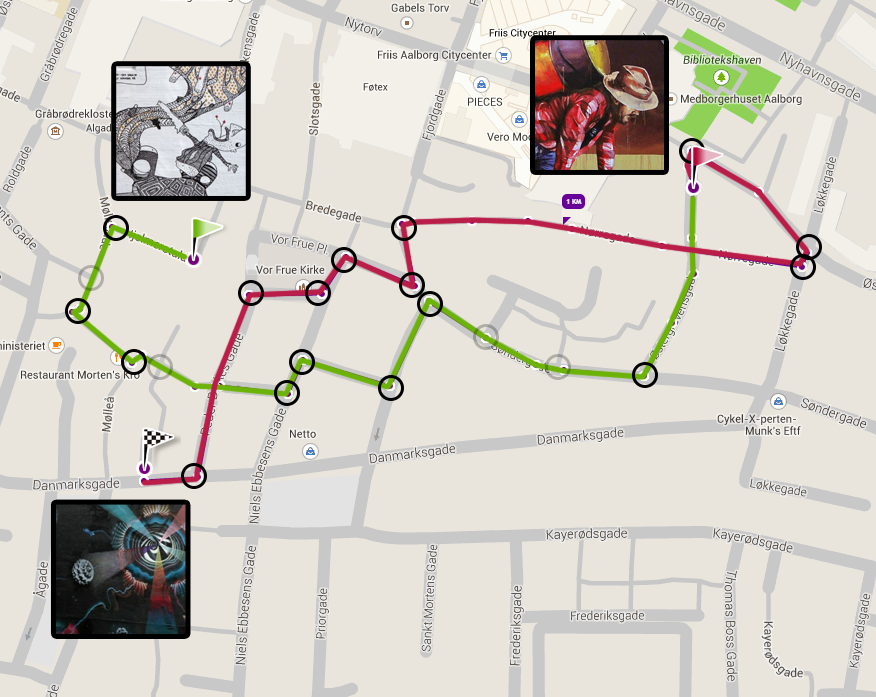
\includegraphics[scale=0.2]{Pics/FinalRoute.png}
\caption{The route between the three street art paintings.}
\label{FinalRoute}
\end{figure}

\subsection{Choice of Navigational Game Activity}
In the process of designing the navigational game activity using landmarks, four initial designs were created as paper prototypes and one was chosen to be used in the game on the basis of three initial tests of the designs. The tests were done using within-subjects design, meaning that each group of participants used a specific navigational game activity for each quarter of the route. The purpose of the tests was to determine which game activity the participants found most enjoyable, based on short semi-interviews conducted between game activities as well as after trying all four activities. The participants of each test were a child in the age group of 8-11 years and the child's parent. We followed the participants during the activities, documenting the tests and interfering if they got lost or had other problems. As the initial designs were paper prototypes with a focus on the navigation, it must be noted that elements of LBGs such as a feedback system, a narrative, activity at POIs, and learning were not a part of the experience in these initial tests.

When designing the four navigational game activities, inspiration was taken from popular children's games, since they are familiar to most children, causing a lower learning curve for the families. Similar game activities were also found in other LBGs, giving inspiration for how they should be used in a LBG. Three navigational game activities were made as variations of matching card games such as \textit{Concentration}\cite{childrensGames}. In these types of games, players specify two or more cards that are alike, among a set of cards, and the goal is typically to be the player with the most matches in the end. In Team Exploration\cite{GamingOnTheMove}, players match pictures in the virtual space to landmarks in the physical space and progress in the game by specifying which pictures belong to certain areas of a map. Similarly, players are given pictures of landmarks in our three matching game activities; \textit{Simple Matching}, \textit{Order Matching}, and \textit{Memory Matching}.

For all four game activities, local landmarks are used to help players choose directions at decision points, and route marks are used along streets to confirm to players that they are walking in the correct direction. In Simple Matching, players are given a set of potential landmarks, where only one of them is a true landmark in their current location. When they spot or match the landmark that is shown on the picture, they go to its position and start matching the next set of pictures. This activity proved to be the easiest of the four and most participants found it to be uninteresting due to its lack of challenge. Order Matching is very similar to Simple Matching, as the only difference is that players have to specify the order in which the presented landmarks occur from their current position. Participants found this activity to be a bit more challenging, however due to the requirement of ordering landmarks, participants sometimes walked back in the direction they came from. Through observation, it was clear that the participants collaborated more in this activity due to the increase in difficulty. In Memory Matching, the landmarks to be ordered are only presented quickly before navigating. When participants then reach the last picture in the set, they are asked to specify the order of landmarks encountered. Through observation and interviews, it was clear that participants found this activity to be the most challenging of all matching activities. This also caused participants to collaborate more, where they e.g. each would remember half of the pictures. Furthermore, participants mentioned that only being able to look at the pictures at certain points, caused them to look more around and notice the environment during navigation.

The last game activity designed was based on riddles, where similar to the game \textit{I Spy}\cite{childrensGames}, players must spot a specific object in the vicinity based on a sentence hinting about attributes of the object. Based on I Spy and the LBG CityTreasure, where riddles are used at POIs, we designed an activity where riddles hint about the next landmark to go to. As in I Spy, the riddles describe attributes of objects through hints.

In the context of landmarks, the riddles describe saliency based on the visual, cognitive or structural attributes of the landmark, either in isolation or in combination. In order for players to confirm that they have found the landmark, they are also given a control question about the landmark with three possible answers. This was a solution to the problem of specifying the players' exact position through GPS, since at the time of designing the activity, it had been observed that accurate positions could not be given through GPS. Furthermore, this control question allows for the possibility of including knowledge about the landmarks in the game activity, thereby supporting pedagogic elements in the game. By being able to confirm if the player has found the landmark, it is possible to create a feedback system in the game. Upon answering the control questions, regardless of the players' answer, a picture of the correct landmark is shown to the players, so they never get lost. Through interviews, it was found that most participants preferred navigation with riddles due to them being the most fun. It was also clear that of all activities, riddles were the most challenging for the participants, mainly because people were unsure of the scale in which the landmarks could be found. This is due to the fact that participants have nothing visual to compare to in opposition to the matching activities. However, it could also be seen that this limitation contributed to the enjoyability of the activity. We also observed that this limitation caused participants to collaborate and in general communicate more during navigation. Based on these results, there were strong indications that navigation using riddles was the most enjoyable activity. For this reason, riddles were chosen as the navigational game activity to be used in our experiment. In order to test the navigational game activity in the context of LBGs, a LBG was developed.

\subsection{Lost on Earth}
\textit{Lost on Earth} builds on the LBG \textit{Monsters Eat Art}\cite{Lynge} made for the iPad. Monsters Eat Art is an interactive museum exploration game, where children in the age group 9-11 find specific artworks based on certain details given. When children find the specific artwork, they use augmented reality (AR) to register the artwork in the game and get feedback. Furthermore, Monsters Eat Art has a narrative with a monster, which eats artworks, and the goal of the game is for the monster to eat a specific group of artworks. A sense of progression is given to the player, since the monster is coloured more black, as it eats the artworks. The monster is also an agent, which gives the player feedback and integrate the narrative throughout the game.

Similarily, in Lost on Earth, the player assists an agent in reaching a specific goal, using artworks, which in our case is the POIs with street art paintings in the city Aalborg. Our game also uses the monster as an agent, and the narrative is built around the monster being stranded on Earth. Since the players' goal is to find landmarks, we designed a narrative that reflects this, by also giving the monster the goal of finding something specific. As the monster is stranded on Earth, it needs to find fuel for its spaceship to fly home. However, the monster is also looking for its friends, which also are stranded on Earth.

Due to the importance of choice and interactive narratives in games, as earlier mentioned, players have the ability to choose whether the monster should look for fuel or friends, which will affect the outcome of the game. These choices are made at the street art paintings. Ideally, different routes should be used for different choices, however to minimize the amount of bias in the experiment, the illusion of choice is given, as the choice will only influence the outcome of the game, not the route to be taken. The choice is made through a dialogue with characters in the street art paintings, which starts as players augment the paintings at the POIs. To incorporate pedagogic elements, information about the painting itself is given through the dialogue, and after augmenting the painting, players unlock access to an info screen about the particular painting. 

In the game activity between POIs, players use riddle solving while navigating, as earlier mentioned. When players start their first riddle, a tutorial introduces how the system works. To incorporate a feedback system, players are given points as they answer correctly on the control questions for the riddles. These points are dependant on the choice made at the previous POI, so for instance in the case that players have chosen to look for fuel, fuel points will be given to the players and vice versa. Whether the monster will fly home or have any friends in the end of the game, will rely on this choice. As seen in the LBG Team Exploration, incorporating limitations in the game such as time, can cause the focus of the game to be more on the hunt itself and not the exploration that takes place in the physical space. For this reason, the limitations used in Lost on Earth are primarily found in the act of navigating itself, where using riddles to navigate is a cumbersome, but also enjoyable way of navigating, as it makes use of the physical space.
\section{Experiment}

To investigate the effects of riddle-solving as the navigation method in a location-based game, we conducted a comparative study between navigating by riddle-solving and navigating by a 2D map with GPS. 

\subsubsection{Hypothesis}

We hypothesized that \textit{riddles as navigational method are more enjoyable than maps.} We came up with the following null hypothesis and its alternative hypothesis. The experiment took place over two weekends in central Aalborg, Denmark. Participants used an iPad 2 3G + WiFi as the platform.

\textbf{H0:} Riddles as navigational method are equal or less enjoyable than maps. 

\hspace{10 mm} \textit{H0: $\mu$EnjoyabilityRiddle $\leq$ $\mu$EnjoyabilityMap}

\textbf{H1:} Riddles as navigational method are more enjoyable than maps.

\hspace{10 mm} \textit{H1: $\mu$EnjoyabilityRiddle $>$ $\mu$EnjoyabilityMap}

\subsubsection{Participants}
We recruited 10 families of 2-6 persons through posters and flyers at schools. 
As the narrative of the game was targeted children, it was a requirement that the families had at least one child in the age range 9-11 year. 17 children participated with ages ranging between the age of 7 and 13 (mean = 10.1, SD = 1.6), 9 females and 8 males. 14 adults participated with ages ranging between the age of 36 and 62 (mean = 42.3, SD = 6.4), 4 females and 10 males.  All participants lived in the city or nearby, and were familiar with the city Aalborg (4 went to the city daily, 5 went to the city weekly, 18 went to the city monthly, 4 went to the city yearly). All participants were familiar using tablet or mobile devices (23 used it daily, 6 used it weekly, 1 used it monthly, 1 used it yearly).


\subsubsection{Materials and Procedure}
The experiment was designed as a within-subjects design with two conditions. (1) A navigational method, where the participants navigated by solving riddles (R) and (2) A navigational method in which the participants used a digital map (M).

These two conditions were counterbalanced with the purpose of reducing the environmental effects met on the route on the results. Participants would either begin with map or riddles, and would end with the navigational method different from the one met in the beginning. 

Three street arts, A, B and C, were a part of the experience. The distance from A to B was 0,9 km and the distance from B to C was 0,9 km. Each condition also had approximately same amount of turns, respectively 8 and 7 turns. Each session lasted between xx min to xx min. One facilitator and one observer would be present during the whole session. The facilitator would explain the participants in using the application before beginning the game, and further help during the game if any difficulties would arise (e.g. participants getting lost). For each session, one of the parents was instructed to wear a GoPro with a harness for recording video, while one of the children carried a bluetooth microphone for recording audio. All parents signed consent forms and filled out demographic questionnaires prior to the experience. We gave the child in the age range 9-11 the iPad, but they were not forced to handle it the whole session. 

LBGs have previously been evaluated using both qualitative and quantitative methods including observational studies, questionnaires and interviews. Morrison et. al. used Flow(kilde), Instrinsic Movation (IMI) [6] and Presence - MEC-SPQ [12] questionnaires and successfully evaluated effects such as enjoyability, motivation and awareness of surroundings by triangulating with video recordings, logs, field notes and transcriptions of interview data. We used the same approach, based on the success of Morrison et al. investigating similar criteria as our study. 

The questionnaire in this study contains questions from the Short Flow State Scale Questionnaire (S-FSS 2), which measures the degree to which flow dimensions characterize the
complete experience. The questionnaire also contains questions from IMI (measures enjoyability, tension, effort and perceived competence) and MEC-SPQ (measures spatial presence, allocated attention and Suspension of Disbelief). Only adults received this questionnaire due to the level of complexity, while children received a simplified questionnaire measuring enjoyability using IMI. Both questionnaires were measured on a likert scale (5-scale), going from 1 (strongly disagree) to 5 (strongly agree). The parents were instructed to help the children to fill out the questionnaire in terms of them having difficulties. 
 
\section{Results}

\subsection{Observations}
During the experiment, an observer walked behind the families and took general notes on the interaction of both conditions. It must be noted that the following observations have not been coded, e.g. through video analysis, but are based on general tendencies.

The biggest differences between the two conditions could be seen in regards to the participants' social behaviour. In general, there was more communication between participants during riddle navigation than during map and the topics were different. During riddles, participants primarily talked about the environment and collaborated to solve the riddles, while during map navigation participants tended to talk about things outside of the game, e.g. one child started talking about his soccer practice. However, this mostly tended to happen on long paths without intersections, as these areas require less attention from users during map navigation. From this, it seems that riddles in general require more attention than maps. For both conditions, collaboration was mostly seen between the child using the iPad and a parent. Here, the parent would act as an assistant to the child and take over the iPad if the child gave up. If there were multiple children, the children not holding the iPad would often had a hard time participating in the navigation and would just follow the group. This indicates that the design does not fully encourage collaboration between multiple players, and it is possible that the collaboration between child and parent naturally arises from the fact that parents are used to assisting their children. During this collaboration however, it was clear that if the riddles were too difficult for the children, but the parents knew the answer, the parents would give their children hints in order for them to solve the riddle. From this, it could be seen that harder riddles encouraged more communication and collaboration.

Regarding the riddle system, it was clear that a better explanation of the system to the participants is needed. Often participants would answer the riddles without going to the position of the previous landmark first, which caused frustration since participants would not be able to find the landmarks used in the riddles. Especially families that used riddle navigation for the second part of the route, had a hard time understanding the system. This indicates that the tutorial built into the system did not provide clear enough instructions. Furthermore, the riddle system is shortly explained by the facilitator in the beginning of the experiment, and this information might have been forgotten as participants reached the second part of the route. 

%This problem could be solved by simply having the facilitator explain the riddle system as the participants start the first riddle

When navigating using the map, the participants' current position on the map was often slow at updating due to the lack of a proper GPS signal. This caused participants to walk down wrong paths, and it could take several minutes for the signal to be re-established, causing confusion in the participants. As a result some participants ended up reaching the destination by taking completely different paths, and in one case, it was necessary for the facilitator to guide the participants.

Finally, it was observed that people in general looked around and paid more attention to the environment when solving riddles than when using a map. During map navigation, the participant holding the iPad primarily looked down on the iPad, and it was mostly at intersections that participants looked around in the environment. It was also observed that especially when the GPS signal was weak during map navigation that participants looked down on the iPad. 	
	
%Children could easily get distracted by things in the environment for both conditions (e.g. dogs)	
%"Nu får vi styr på Aalborg"
\subsection{Questionnaires}
We used the Wilcoxon Signed-Rank test, based on the nature of ordinal values and due to the sample had been exposed to two conditions (riddle solving and map).

All participants found the system using Riddles significantly more intrinsic motivating (IMI) than maps(See Table \ref{my-label1}). Assessing IMI, we found that enjoyability and effort scored significantly higher for Riddles compared to Maps. Riddles also received a significantly higher score than Maps concerning total Flow. No significant difference was found for Presence, but Riddles was still favoured in terms of its score. 

\begin{table}[h]
\caption{Questionnaire items showing significant differences between Riddle navigation and map navigation}
\label{my-label1}
\begin{tabular}{lll}
\hline
\multicolumn{1}{|l|}{\textbf{\begin{tabular}[c]{@{}l@{}}Item and Wilcoxon\\ Signed-Rank Test\end{tabular}}} & \multicolumn{1}{l|}{\textbf{\begin{tabular}[c]{@{}l@{}}System\\ with higher\\ mean\end{tabular}}} & \multicolumn{1}{l|}{\textbf{\begin{tabular}[c]{@{}l@{}}System\\ with lower\\ mean\end{tabular}}} \\ \hline
\multicolumn{3}{|l|}{\cellcolor[HTML]{EFEFEF}\textit{Item related IMI for \textbf{all participants}}}                                                                                                                                                                                                                                    \\ \hline
\multicolumn{1}{|l|}{IMI - total(**)}                                                                       & \multicolumn{1}{l|}{\begin{tabular}[c]{@{}l@{}}Riddle\\ Mean=4.31\end{tabular}}                  & \multicolumn{1}{l|}{\begin{tabular}[c]{@{}l@{}}Map\\ Mean=3.64\end{tabular}}                    \\ \hline
\multicolumn{1}{|l|}{IMI - Enjoyment(**)}                                                                   & \multicolumn{1}{l|}{\begin{tabular}[c]{@{}l@{}}Riddle\\ Mean=4.49\end{tabular}}                  & \multicolumn{1}{l|}{\begin{tabular}[c]{@{}l@{}}Map\\ Mean=3.46\end{tabular}}                    \\ \hline
\multicolumn{1}{|l|}{IMI - Pressure(-)}                                                                     & \multicolumn{1}{l|}{\begin{tabular}[c]{@{}l@{}}Map\\ Mean=2.11\end{tabular}}                     & \multicolumn{1}{l|}{\begin{tabular}[c]{@{}l@{}}Riddle\\ Mean=1.78\end{tabular}}                 \\ \hline
\multicolumn{1}{|l|}{IMI - Effort(*)}                                                                       & \multicolumn{1}{l|}{\begin{tabular}[c]{@{}l@{}}Riddle\\ Mean=4.30\end{tabular}}                  & \multicolumn{1}{l|}{\begin{tabular}[c]{@{}l@{}}Map\\ Mean=3.68\end{tabular}}                    \\ \hline
\multicolumn{1}{|l|}{IMI - Perceived Competence(-)}                                                         & \multicolumn{1}{l|}{\begin{tabular}[c]{@{}l@{}}Riddle\\ Mean=4.13\end{tabular}}                  & \multicolumn{1}{l|}{\begin{tabular}[c]{@{}l@{}}Map\\ Mean=3.68\end{tabular}}                    \\ \hline
\multicolumn{3}{|l|}{\cellcolor[HTML]{EFEFEF}\textit{Item related Flow only for \textbf{adults}}}                                                                                                                                                                                                                                             \\ \hline
\multicolumn{1}{|l|}{Flow - total(*)}                                                                       & \multicolumn{1}{l|}{\begin{tabular}[c]{@{}l@{}}Riddle\\ Mean=3.85\end{tabular}}                  & \multicolumn{1}{l|}{\begin{tabular}[c]{@{}l@{}}Map\\ Mean=3.60\end{tabular}}                    \\ \hline
\multicolumn{3}{|l|}{\cellcolor[HTML]{EFEFEF}\textit{Item related Presence only for \textbf{adults}}}                                                                                                                                                                                                                                         \\ \hline
\multicolumn{1}{|l|}{Presence - total(-)}                                                                   & \multicolumn{1}{l|}{\begin{tabular}[c]{@{}l@{}}Riddle\\ Mean=3.07\end{tabular}}                  & \multicolumn{1}{l|}{\begin{tabular}[c]{@{}l@{}}Map\\ Mean=2.95\end{tabular}}                    \\ \hline
\multicolumn{3}{l}{\begin{tabular}[c]{@{}l@{}}Note: (-) = p\textgreater.05 and (*) = p\textless.05 and (**) = p\textless.01\\ IMI, Flow and Presence 1-5 scale\end{tabular}}                                                                                                                                      
\end{tabular}
\end{table}

We found significant differences when assessing individual questions from the questionnaire (See Table \ref{my-label}). All participants especially found the Riddle system significantly more fun and less boring compared to the map version. We observed that riddles served a potential of including multiple family members, which  accommodate the fact that all participants had a enjoyable experience. 

Adults found the riddles significantly more rewarding and had the feeling of the time moving faster compared to the map version. These two questions specifically assesses the dimension on having an autotellic experience and the sense of time transformation. As flow involves nine dimensions, these two were the only dimensions to reveal a significant difference. Other dimensions of flow favoured Riddles, or were closely tied with Maps (0.05 score difference between R and M), except for a flow question revolving on clear goals. Our questionnaire revealed that test participants found the Map system had more clear goals (R =3.31, M =3.83, p=.174). As the result is not significant, it is however observed that the Map did not require much training, and henceforth more intuitive than what we observed with the Riddle system. However, participants still favoured the Riddle system despite these difficulties. 

Children thought they were significantly better at navigating with Riddles, rather than using a maps. We found that children considered maps more challenging from the questionnaire which could provide an explanation on the matter, but this was not founded significant (R =2.82, M =3.33, p=.177).
 
We performed a multiple ordinal regression analysis on the questions from Table \ref{my-label}, whether age, gender, condition order or group size served as predictors for the results. In all cases, the results stayed significant, but the condition order was revealed to have a significant impact on several of the questions concerning IMI. 

Due to the condition order, the selection of Riddles was different, as well as the route described on the Map. Different attractions on the route would be met differently based on the condition order, and eventually provide a different experience. 

\begin{table}[h]
\caption{Questionnaire items showing significant differences between Riddle navigation and map navigation}
\label{my-label}
\begin{tabular}{|l|l|l|}
\hline 
\textbf{\begin{tabular}[c]{@{}l@{}} Item and Wilcoxon \\ Signed-Rank Test\end{tabular}} & \textbf{\begin{tabular}[c]{@{}l@{}}System\\ with higher \\ mean\end{tabular}} & \textbf{\begin{tabular}[c]{@{}l@{}}System \\ with lower \\ mean\end{tabular}} \\ \hline
\rowcolor[HTML]{EFEFEF} 
\hline
\multicolumn{3}{|l|}{\cellcolor[HTML]{EFEFEF}\textit{Items related\textbf{ all participants}}} \\ \hline
\begin{tabular}[c]{@{}l@{}}IMI: I thought navigating\\ was fun (**)\end{tabular} & \begin{tabular}[c]{@{}l@{}}Riddle\\ Mean=4.48\end{tabular} & \begin{tabular}[c]{@{}l@{}}Map\\ Mean=3.42\end{tabular} \\ \hline
\begin{tabular}[c]{@{}l@{}}IMI: I thought navigating\\  was boring (R) (**)\end{tabular} & \begin{tabular}[c]{@{}l@{}}Map\\ Mean=2.14\end{tabular} & \begin{tabular}[c]{@{}l@{}}Riddle\\ Mean=1.41\end{tabular} \\ \hline
\begin{tabular}[c]{@{}l@{}}Flow: My attention was\\ focused on navigating (*)\end{tabular} & \begin{tabular}[c]{@{}l@{}}Riddle\\ Mean=4.16\end{tabular} & \begin{tabular}[c]{@{}l@{}}Map\\ Mean=3.66\end{tabular} \\ \hline
\rowcolor[HTML]{EFEFEF} 
\multicolumn{3}{|l|}{\cellcolor[HTML]{EFEFEF}\textit{Items related only \textbf{adults}}} \\ \hline
\begin{tabular}[c]{@{}l@{}}Flow: I found the experience\\  highly rewarding (*)\end{tabular} & \begin{tabular}[c]{@{}l@{}}Riddle\\ Mean=3.93\end{tabular} & \begin{tabular}[c]{@{}l@{}}Map\\ Mean=3.15\end{tabular} \\ \hline
\begin{tabular}[c]{@{}l@{}}IMI: I enjoyed\\  navigating a lot (*)\end{tabular} & \begin{tabular}[c]{@{}l@{}}Riddle\\ Mean=4.29\end{tabular} & \begin{tabular}[c]{@{}l@{}}Map\\ Mean=3.46\end{tabular} \\ \hline
\begin{tabular}[c]{@{}l@{}}Flow: It felt like time\\  went by quickly (*)\end{tabular} & 
\begin{tabular}[c]{@{}l@{}}Riddle\\ Mean=4.54\end{tabular} & \begin{tabular}[c]{@{}l@{}}Map\\ Mean=3.69\end{tabular} \\ \hline
\rowcolor[HTML]{EFEFEF} 
\multicolumn{3}{|l|}{\cellcolor[HTML]{EFEFEF}\textit{Items related only \textbf{children}}} \\ \hline
\begin{tabular}[c]{@{}l@{}}IMI: I thought I was pretty\\  good at navigating (*)\end{tabular} & 
\begin{tabular}[c]{@{}l@{}}Riddle\\ Mean=4.41\end{tabular} & \begin{tabular}[c]{@{}l@{}}Map\\ Mean=3.73\end{tabular} \\ \hline
\multicolumn{3}{l}{\begin{tabular}[c]{@{}l@{}}Note: (*) = p\textless.05 and (**) = p\textless.01. \\ IMI and Flow 1-5 scale\end{tabular}}
\end{tabular}
\end{table}
   
We can reject our null hypothesis, stating that riddles as navigational method are more enjoyable than maps.

\subsection{Interviews}
From the interview data, we found that 5 out of 22 children expressed preference towards using maps. One parent mentioned she also preferred map, saying \textit{"It is just always fun to follow a map"}. This parent explained that they were unsure about what to do during the riddle-based navigation and could not remember what they had been told during the instructions. 

Another parent mentioned that map was easy and did not make one aware of the surroundings, because the focus was on walking. In general, we found different opinions on whether the different navigational methods made people aware of the surroundings. One parent clearly stated the the children were not interested in the map at all. In line with several other test participants this parent expressed that it was fun to notice things in the environment they usually do not notice when walking by, making it an optimal method for tourists. Opposed to that opinion, another parent expressed that she focused more on navigating than noticing things in the environment. With riddles, one parent felt that the attention was on the next location to go to, while the map made the participant more aware of the city, because there was more time to look around in the surroundings. 

When asked if they would use riddles as navigational method, if they were to use it in another city, all test participants agreed and answered yes. Some thought it would be a more fun way of learning the city, finding the way and that it would make it possible to see the city in a different way. However, interview data also clearly revealed that several participants would have enjoyed it more, if the riddles were about more interesting landmarks that gave the possibility to learn more e.g. about the city. Preferably this should be done with the children in mind and a few parents proposed a system that can be adjusted depending on, whether they had any children and adjusted content according to the children’s age. Riddles as navigational method was described as \textit{"fun if you have time for it"} by one parent. This reflected the results from the questionnaires. 

The most used word to describe riddle-based navigation was "fun" (11 of 29 words). Other words included exciting, challenging, different, educational and inspiring. Some participants thought it was fun to answer the questions after the riddles, particularly one child mentioned that it was fun to be able to answer correctly to questions. Results from the log show a high tendencies of correct answers to control questions. In average 96,9 percentage of the control questions across all sessions were answered correctly. One also expressed that it was fun to find the matching pictures in the environment. 

One parent mentioned that the fun part in the riddle-based navigation was to help each other and agree on what they have seen in the environment. Several parents had a similar opinion and stated that they enjoyed collaborating and discussing the answers with the other family members. One parent said it was fun with riddles, 

\begin{quote}
    "(...) because there was something to discuss. Of course you can also discuss what way to go with the map, but that just gave a different experience."
\end{quote}

In terms of group dynamics, it was mentioned that primarily the one with the device was in control, making it a less collaborative experience. One parent mentioned that they collaborated more, when navigating using riddles and not as much with the map. In order to make it more collaborative, one of the participants suggested making the riddles more difficult, encouraging the participants to help each other. This statement supports the experience of another parent, who mentioned that they only collaborated when there was any doubt, otherwise they just followed the child, who was mostly in charge of the device. 

The interview data revealed a tendency to let the child control the device, which was described as following by one parent,  

\begin{quote}
    "Then one finds out about something and the other finds out about something else. I 
felt I gave much of the control to Mikki (the child), because I wanted him to think it 
was fun."
\end{quote}
 
In one family, the parent stated that it was much more fun for them both, when the child had the device, because the child was better at using the map and tablets in general.
\section{Conclusion}
In this study, we investigated the effects of riddle solving as a navigational method in a location-based game experience for families. We compared this navigational method with a 2D map, which is a common navigational method to get from one POI to another in location-based games. We found significant results indicating that riddle-solving as a navigational method is more enjoyable than a 2D map. Though perhaps not being a more intuitive navigational method than 2D maps, riddle-solving clearly suits the scope of location-based game experiences, as it makes use of the physical space to navigate from one POI to another, while also adding more enjoyment to the experience. We recommend looking into using this or similar approaches to create not only enjoyable, but also educational experiences. 
\section{Discussion}
%One of the main objectives of this study was to design a navigational method in which an interplay between the physical and virtual world occurs. We proposed a navigational method that incorporated location-based game activities, where participants navigated by solving riddles in the virtual space about landmarks in the physical space. 
Results from our study clearly shows that riddle solving is a more enjoyable way of navigating than a 2D digital map. However, findings from interviews with the families revealed that some children also enjoyed navigating with maps. Children were challenged using the map as well as riddles for navigation, perhaps because they are not used to any of the navigational methods. We found that children thought they were better at navigating with riddles than maps. Similarly, parents were significantly more in flow with riddle-based navigation than with the 2D map, meaning there was a better challenge-skill balance with riddle-based navigation. One of the explanations could be that parents were less challenged by using maps, as they are used to navigate with maps, while riddle-based navigation was just as novel an experience for the parents as for the children. Particularly in the beginning, we observed that our test participants experienced difficulties understanding the rules of the riddle-based navigation, which was supported by the fact that participants spent most time on the first riddle. Questionnaire data also  supported this, as riddles scored lower on clear goals. We assume that maps were less challenging to use, despite of the GPS problems that occured during the experiment, and therefore that challenge was one of the reasons why riddle-based navigation scored higher on enjoyment. Furthermore, we also found that children enjoyed answering questions, getting feedback. This supports that incorporating game activities in a location-based experience like this, makes it more enjoyable for the players - even if it is more challenging and unneccessary obstacles have to be met. 

%The average completion time of solving one riddle across all sessions, reveals the first riddle as most challenging (in terms of time spent) indicating only a short learning curve and that collaboration is most needed only at the first riddle. 

We found no significant results about presence, though riddle-based navigation scored higher on making the participants aware of their surroundings. One of the main objectives of this study was to create a navigational method with a stronger interplay between the physical and virtual space. Interview data revealed different opinions on whether participants were more or less aware of the surroundings using riddle-based navigation, where landmarks are used to navigate between POIs. With map navigation, some participants felt that they were more free to notice things in the surroundings, while riddle-based navigation only made some more aware of the landmarks. This might have been due to different levels of engagement and roles that the participants took, but also the more collaborative approach some had in the families during riddle solving.   

%Others emphasized that one of the qualities of riddle-based navigation was that it made one aware of things that otherwise would have gone unnoticed.

Despite not being the main focus of this study, we observed some interesting elements in terms of social interaction among participants. Even though we did not find any statistically significant results supporting that participants helped each other more during riddle-based navigation, compared to a map, we found that riddle-based navigation has potential in motivating groups of people, making it a enjoyable group experience rather just a matter of getting from A to B, where on person is in charge. We observed that participants discussed more and that topics revolved around solving the riddles, discussing the landmarks and not on topics outside the activity, as it was the case with map navigation. Though this requires a more thorough analysis of the interaction among the participants, we hypothesize that riddle-based navigation has potential in supporting learning e.g. about landmarks or developing skills in terms of exploration, particularly in group context. Even though enjoyment is the main objective of most LBGs as mentioned by Avouris \& Yiannoutsou \cite{LBG_Review}, we recommend looking into riddle-based navigation or similar approaches for informal learning, as this study has shown the potential in incorporating the time spent navigating into the overall enjoyable experience of a location-based game. 

%However, we found no statistically significant results in terms of participants helping each other more during riddle-based navigation. 

%- Social interaction --> Potential in motivating groups of people, making it a family experience rather than a matter of getting from A to B. Potentials in terms of learning about the environment. 

%\cite{AugmentingAudioMessages} \cite{Carrigy:2010:DEP:1868914.1868929} \cite{DesigningMobileARI} \cite{GamingTourism} \cite{HideAndSeek} \cite{InterdisciplinaryCriticism} \cite{JCAL:JCAL316} \cite{Klemmer:2002:WSC:503376.503378} \cite{LostLab} \cite{Mather:2000:MUT} \cite{Savannah} \cite{Schwartz:1995:GBF} \cite{StoryTrek} \cite{TheoreticalAndMethod} 

% Balancing columns in a ref list is a bit of a pain because you
% either use a hack like flushend or balance, or manually insert
% a column break.  http://www.tex.ac.uk/cgi-bin/texfaq2html?label=balance
% multicols doesn't work because we're already in two-column mode,
% and flushend isn't awesome, so I choose balance.  See this
% for more info: http://cs.brown.edu/system/software/latex/doc/balance.pdf
%
% Note that in a perfect world balance wants to be in the first
% column of the last page.
%
% If balance doesn't work for you, you can remove that and
% hard-code a column break into the bbl file right before you
% submit:
%
% http://stackoverflow.com/questions/2149854/how-to-manually-equalize-columns-
% in-an-ieee-paper-if-using-bibtex
%
% Or, just remove \balance and give up on balancing the last page.
%
\balance

\bibliographystyle{acm-sigchi}
\bibliography{references}
\end{document}
